\documentclass[11pt,a4paper,titlepage, ngerman]{article}

\usepackage[utf8]{inputenc}	% Diese Pakete sind
\usepackage[T1]{fontenc}		% für die Verwendung 
\usepackage{ngerman}			% von Umlauten im tex-file
\usepackage{lmodern}			% Schriftart, die am Bildschirm besser lesbar ist
\usepackage{graphicx}			% Zum Einbinden von Formeln
\usepackage{url}					% Zur Darstellung von Webadressen
\usepackage{siunitx}
\usepackage{amsmath}			% für equation*
\usepackage{subcaption}
\usepackage{wrapfig}

\begin{document}
%	\setlength{\parindent}{0em} 
	
	\begin{titlepage}
		\centering
		{\scshape\LARGE Versuchsbericht zu \par}
		\vspace{1cm}
		{\scshape\huge E4 -- Kennlinien\par}
		\vspace{2.5cm}
		{\LARGE Gruppe 10 Mi\par}
		\vspace{0.5cm}
		{\large Alex Oster (E-Mail: a\_oste16@uni--muenster.de) \par}
		{\large Jonathan Sigrist (E-Mail: j\_sigr01@uni--muenster.de ) \par}
		\vfill
		durchgeführt am 8.11.2017\par
		betreut von\par
		{\large David \textsc{Pahl}}
		
		\vfill
		
		%TODO Grafikbeschriftungen an die Messung/Versuch anpassen und keine nummer
		
		{\large \today\par}
	\end{titlepage}
		
	\tableofcontents
	
	\newpage
	
	\section{Kurzfassung}
		
		In diesem Bericht befassen wir uns mit Kennlinien. Eine Kennlinie ist die Kurve, die entsteht, wenn man die Spannung gegen den Strom aufträgt. Aus dem Ohm'schen Gesetz $U=RI$ bzw. $I = \frac{1}{R}U $ ergibt sich, dass diese durch den Widerstand dargestellt wird und bei konstanten Widerständen linear verläuft.
		
		Wir betrachten im Folgenden zwei Versuchen, die uns verschiedenen Arten von Widerständen näher bringen sollen.
		Diese hängen unter anderem von der Temperatur, den Materialien und der Bauteilgeometrie ab.
		
		In dem ersten Versuch betrachten wir fünf verschiedene Arten von Widerständen. Eine einfache Diode, eine Zenerdiode, einen NTC-Widerstand, eine Glüh- und eine Glimmlampe. Wir messen hierbei den Strom in Abhängigkeit von der Spannung und werten die Ergebnisse aus. Dazu gehen wir auf die Funktionsweise von (dotierten) Halbleitern und Gasentladungen ein. 
		
		Die Abhängigkeit des Widerstands von der Temperatur wird dann in dem zweiten Versuch für einen Kupferdraht betrachtet.
		Hierzu erhitzen wir diesen Draht in Öl, lassen ihn danach abkühlen und messen durchgehend seinen Widerstand mit Hilfe einer Wheatstone'schen Brücke. Unsere Ergebnisse für den Kupferdraht verknüpfen wir dann mit der elektrischen Leitfähigkeit von Metallen.

	\section{Versuch 1: Strom-Spannungs-Charakteristik}
		
		In diesem Versuch betrachten wir die Kennlinien von verschiedenen Bauteilen. Dafür messen wir den Strom und tragen diesen gegen unsere Eingangsspannung auf. Den sich daraus ergebenen Verlauf, die Kennlinie, erklären wir dann im Sachverhalt. 
		
		\subsection{Methoden} 
		
		Der Versuchsaufbau ist in Abb. \ref{Schaltskizze1} skizziert. Dabei fließt der Strom nur über jeweils eine Teilschaltung \textbf{a)} bis \textbf{e)}. 
		Da die Spannungsquelle keine genaue Angabe der Eingangsspannung liefert, messen wir diese mit einem Multimeter über das relevante Bauteil.
		Den Strom messen wir mit einem zweiten Multimeter, welches in Reihe geschaltet ist.
		
		Für die Teilversuche \textbf{a)} bis \textbf{d)} verwenden wir Eingangsspannungen im Bereich von \SIrange{0}{20}{\V} und für die Glimmlampe in \textbf{e)} Eingangsspannungen von \SIrange{0}{150}{\V}.
		
		\begin{figure}
			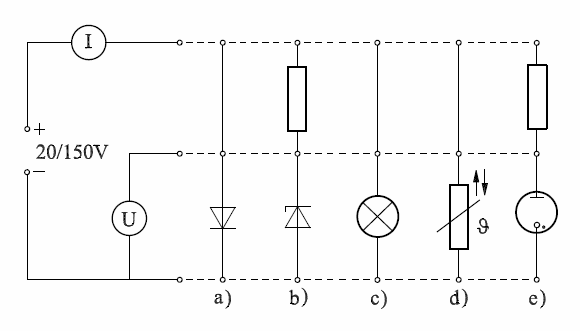
\includegraphics[width=\textwidth]{Versuch1.png}
			\caption{Schaltskizze zu Versuch 1}
			\label{Schaltskizze1}
		\end{figure}

		\subsection{a) Diode in Durchlassrichtung} 
			\label{a)}
			
			\subsubsection*{Diode}
				\label{Diode}
								
				Eine Diode ist ein Bauteil, mit dem Ströme nur von einer Richtung durchgelassen werden.
				Diesen Effekt erhält man, wenn man einen Halbleiter mit einem Element aus der dritten Hauptgruppe dotiert (p-Leiter) und einen anderen mit einem Element aus der fünften Hauptgruppe (n-Leiter) und diese aneinander grenzen lässt.
				Hierbei entsteht eine Raumladungszone im Übergangsbereich, da die Elektronen des n-Leiters zu dem p-Leiter wandern.
				Da in diesem Übergangsbereich weniger freie Ladungsträger sind, als im restlichen Leiter, nimmt die Leitfähigkeit an dieser Stelle stark ab.
				

				Legt man an den positiven Pol, also den n-Leiter eine äußere Spannung an, so vergrößert sich der Übergangsbereich.
				Bei umgekehrter Polung hingegen, verkleinert sich dieser und verschwindet bei außreichend hoher Spannung komplett, sodass der Strom durch den Leiter fließen kann. 
			
			\subsubsection*{Messung}
				
				Unsere Messwerte ergaben, wie in Abb. \ref{KL a} zu sehen ist, dass die Kennlinie bei einer Diode in Durchflussrichtung exponentiell verläuft.
				Einen messbaren Strom erhielten wir erst ab ca. \SI{0.5}{\V} und es ließen sich ab ungefähr \SI{0.72}{\V} keine weiteren Werte messen. Der Regler für die Spannungsquelle war bereits am Anschlag. Im Bereich \SIrange{0,65}{07}{\V} wurde das Einstellen besonders schwierig.
				
				\begin{figure}
					\centering
					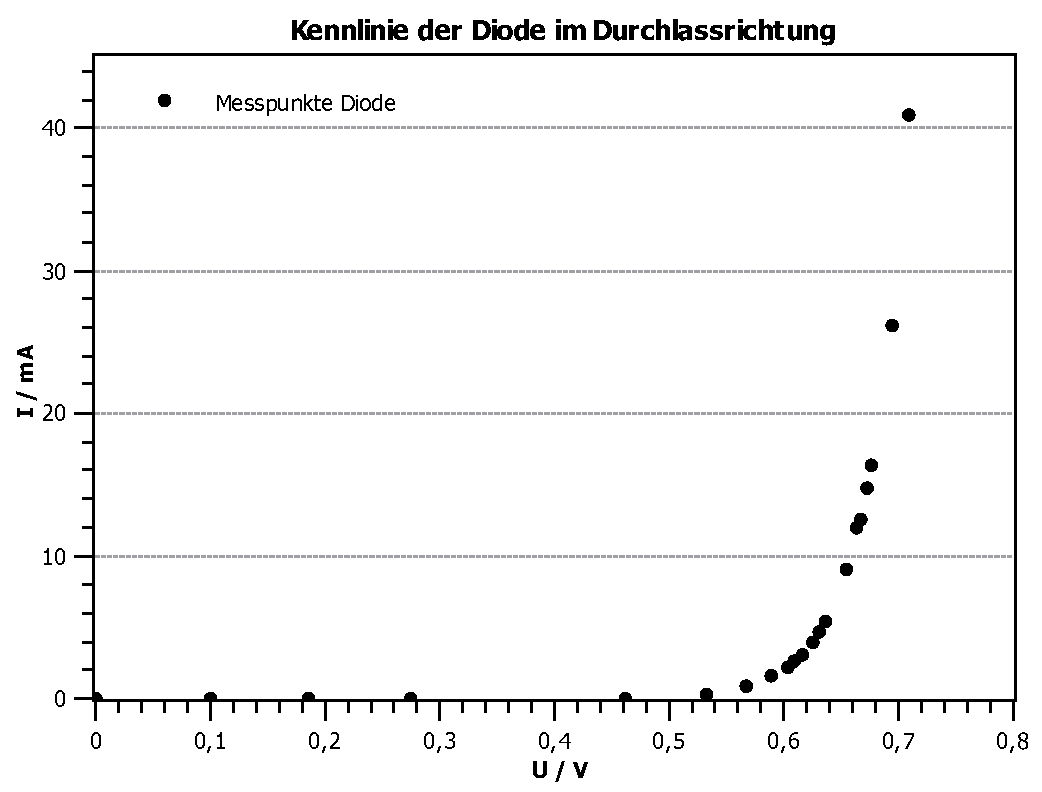
\includegraphics[width=\textwidth]{KennlinieDiode.pdf}
					\caption{Messung zu Versuch 1a)}
					\label{KL a}
				\end{figure}
			
			\subsubsection*{Schlussfolgerung}
							
				Unsere Ergebnisse deuten darauf hin, dass mindestens \SI{0.5}{\V} nötig sind, um den Übergangsbereich der Diode soweit zu verkleinern, dass überhaupt ein Strom fließen kann. 				
				Dass sich ab ca. \SI{0.72}{\V} keine weiteren Werte messen  ließen, lag daran, dass keine höheren Eingangsspannungen möglich waren. Hierbei könnte der Innenwiderstand des Netzteils eine Rolle spielen.

				Die Größe des Übergangsbereichs steht in direktem Zusammenhang mit dem Widerstand.
				Denn bei einer höheren Spannung ist auch der Übergangsbereich kleiner und freie Ladungsträger können ihn leichter passieren.
				Der Widerstand wird also geringer.
				
				Dieser Sachverhalt wird durch den exponentiellen Verlauf der von uns gemessenen Kennlinie unterstützt.
				Somit entspricht unser Ergebnis den Erwartungen.
				
		\subsection{b) Zenerdiode} 
			
			Die Zenerdiode funktioniert ähnlich wie die in \ref{Diode} beschriebene Diode, nur dass bei ihr auch in Sperrrichtung Strom fließen kann.
			Dies geschieht durch das Kleiner-werden der Potentialbarrieren bei hochdotierten p-n-Übergängen, wenn hohe Spannungen angelegt werden.
			Hierbei kommt es zu dem quantenmechanischen Tunneleffekt, durch welchen Valenzelektronen in das Leitungsband gelangen.
			Es bildet sich ein Durchbruchstrom, welcher die Diode nicht zerstört, wie es bei einem Lawinendurchbruch der Fall wäre.
			
			\subsubsection*{Messung}
			
				 \begin{itemize}
				 	
				 	\item Sperrrichtung: 
				 	
				 	In Abb. \ref{KL b1} erkennt man, dass wir auch hier einen exponentiellen Verlauf der Kennlinie gemessen haben. 				 	
				 	Anders als in der vorausgehenden Messung, fließt hier jedoch erst ab ca. \SI{2.6}{\V} ein Strom und wir konnten dieses mal bis ungefähr \SI{5}{\V} einen Strom messen.
				 	Damit liegt die Durchbruchspannung deutlich über der Durchlassspannung.
				 	
				 	\begin{figure}
				 		\centering
				 		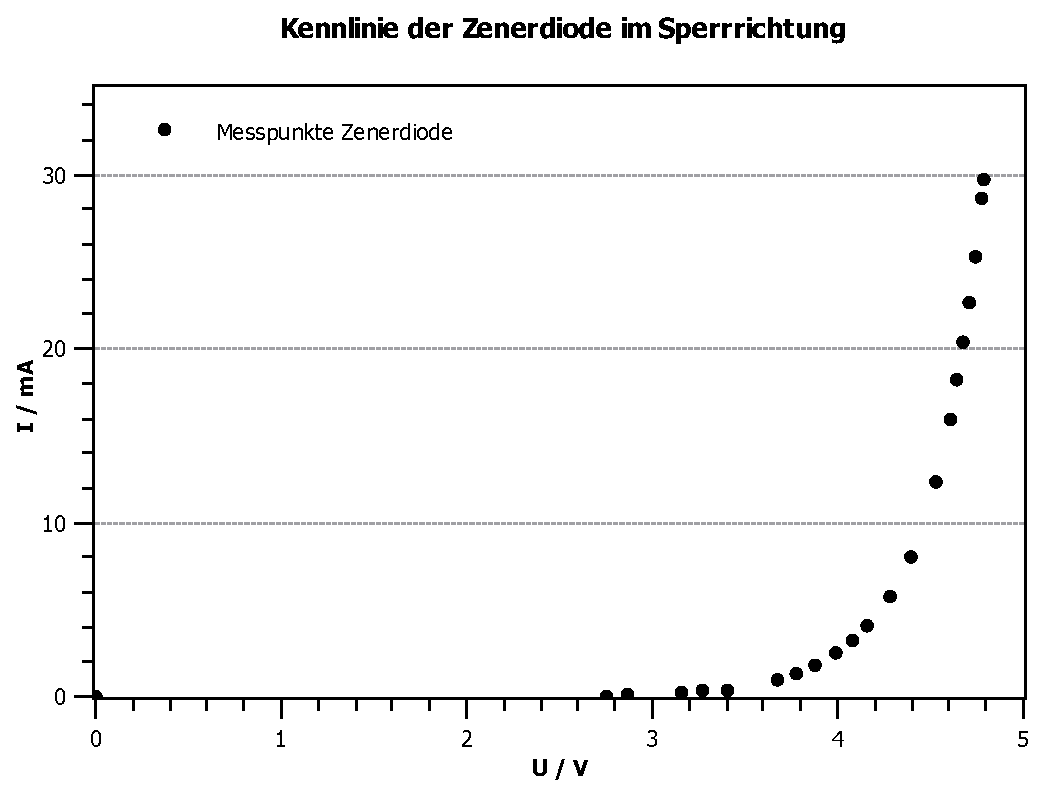
\includegraphics[width=\textwidth]{KennlinieZenerdiodeSperrrichtung.pdf}
				 		\caption{Erste Messung zu Versuch 1b)}
				 		\label{KL b1}
				 	\end{figure}
				 	
				 	\item Durchlassrichtung:  
				 	
				 	Diese Messung verlief analog zu der in \ref{a)} durchgeführten Messung, wie in Abb. \ref{KL b2} zu sehen.
				 	Auch hier beträgt die Durchlassspannung ca. \SI{0,55}{\V}.

				 	Verglichen mit Abb. \ref{KL a}, ist diese gleichmäßiger und der zu erkennende exponentielle Anstieg wirkt ein wenig stärker.
				 	
				 	\begin{figure}
				 		\centering
				 		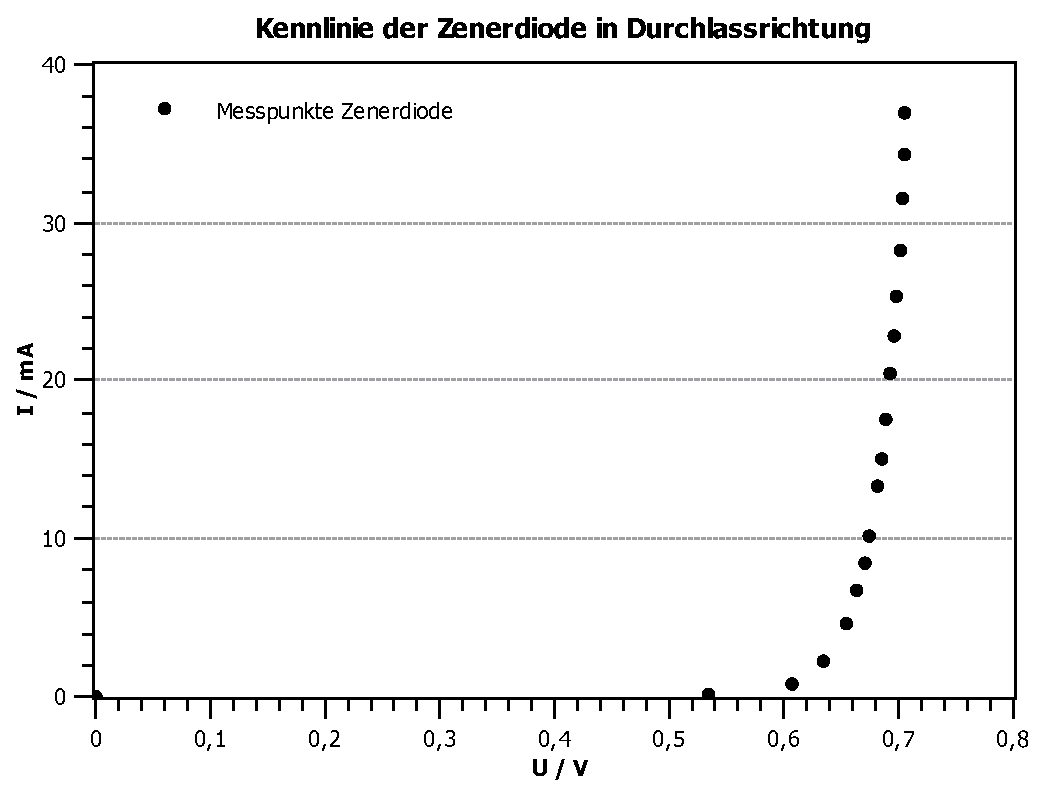
\includegraphics[width=\textwidth]{KennlinieZenerdiodeDurchlassrichtung.pdf}
				 		\caption{Zweite Messung zu Versuch 1b}
				 		\label{KL b2}
				 	\end{figure}
				 					 	
				\end{itemize}
											
			\subsubsection*{Schlussfolgerung}
				
				Die Ergebnisse dieser Messung bezüglich der Durchlassrichtung stehen in direktem Zusammenhang zu dem Ergebnis aus \ref{a)}. 
				Für die Sperrrichtung hingegen ermitteln wir, dass die benötigte Spannung für einen Stromfluss bei ca. \SI{2.6}{\V} liegt. 
				
				Verglichen mit den \SI{0.5}{\V} in Durchflussrichtung ist dies ein beachtlicher und zu erwartender Unterschied.
				Im Gegenzug zu der Verkleinerung des Übergangsbereichs der Diode fließt in Sperrrichtung, wenn überhaupt, nur der Durchbruchstrom und für diesen benötigt man hohe Spannungen. 
				
				Dass auch in Sperrrichtung die Kennlinie exponentiell verläuft, hat einen ähnlichen Grund, wie in Durchflussrichtung.
				Denn mit höheren Spannungen lösen sich auch mehr Elektronen aus dem Valenzband des p-Leiters und folglich ist der Durchbruchstrom stärker.
				Der Widerstand wird also auch hier mit höherer Spannung kleiner. 
				
		\subsection{c) Glühlampe} 
			
			Bei der Glühlampe fließt der Strom durch einen Glühdraht.
			Dieser erwärmt sich dabei und beginnt zu glühen.
			Wir betrachten also nun, wie sich der Widerstand nach Inbetriebnahme der Glühlampe ändert.
			Dazu messen wir den Strom wie bisher und tragen ihn gegen die Spannung auf.
			Um die Änderung des Widerstandes besser zu betrachten tragen wir zudem noch den Widerstand gegen die Spannung auf, wobei sich dieser aus dem Ohm'schen Gesetz ($R = U / I$) und der vorausgegangen Strommessung ergibt.  
			
			\subsubsection*{Messung}
				
				Die Kennlinie der Glühlampe verläuft zunächst krumm, richtet sich im späteren Verlauf jedoch annähernd linear aus. Wir beobachten, dass die Glühlampe ab ca. \SI{2.6}{\V} anfängt schwach zu glühen. In Abb. \ref{KL c} ist zu sehen, dass die Kennlinie sich in diesem Bereich beginnt sich linear auszurichten.
				Der Graph in Abb. \ref{R c} zeigt, dass auch ohne angelegte Spannung, also bei Zimmertemperatur, ein Widerstand vorliegt. Der weitere Verlauf ist annähernd linear, wobei sich die Steigung bei ca. \SI{2}{\V} ändert (kleiner wird).
				
				Der letzte messbare Wert lag hier bei ca. \SI{7.2}{\V}.
				
				\begin{figure}
					\centering
					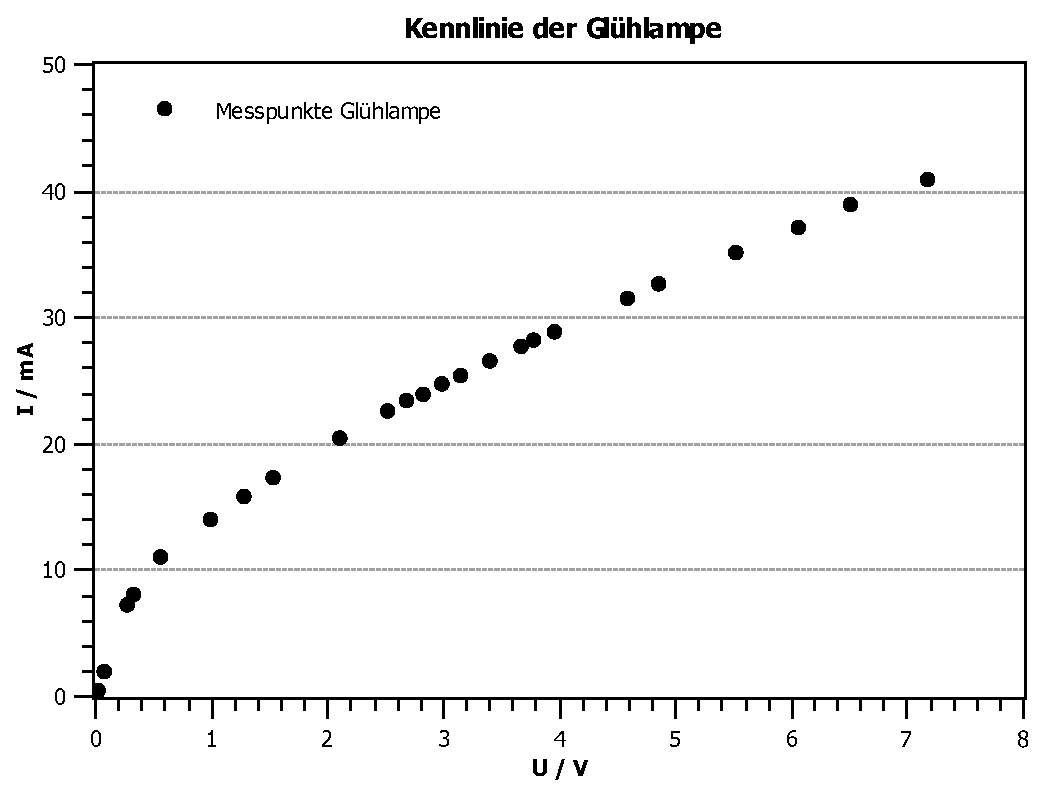
\includegraphics[width=\textwidth]{KennlinieGluehlampe.pdf}
					\caption{Messung zu Versuch 1c)}
					\label{KL c}
				\end{figure}
				\begin{figure}
					\centering
					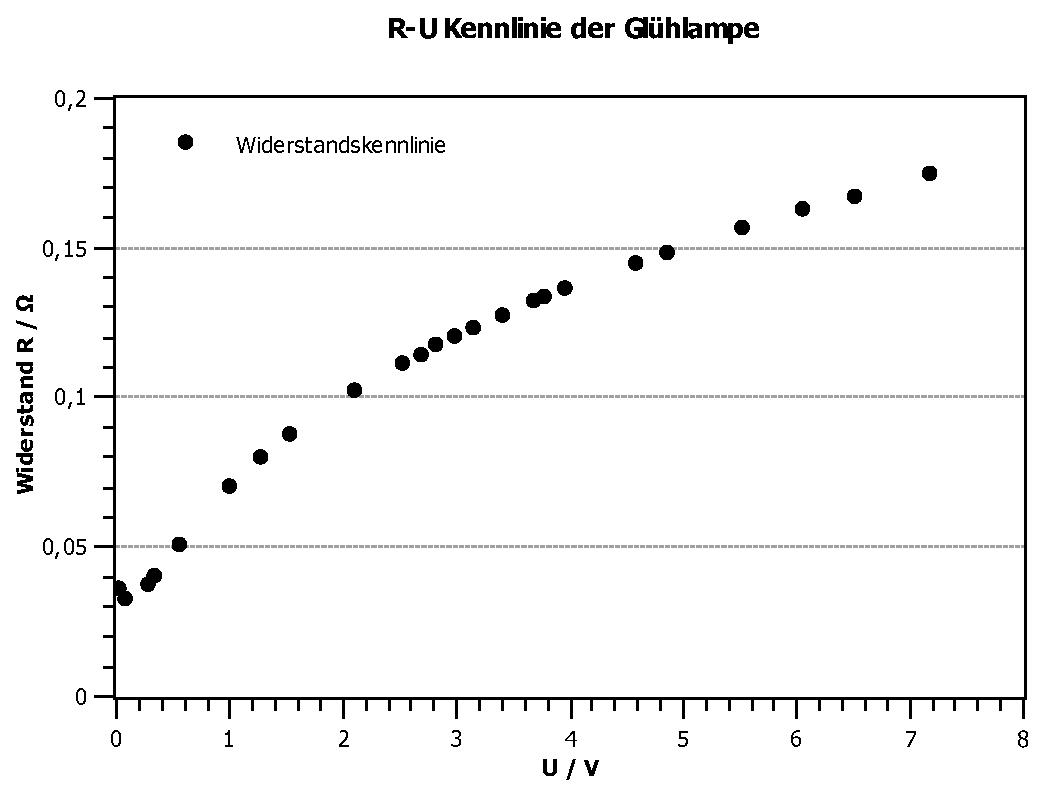
\includegraphics[width=\textwidth]{KennlinieGluehlampeWiderstand.pdf}
					\caption{Widerstand in Abhängigkeit der Spannung}
					\label{R c}
				\end{figure}
			
			\subsubsection*{Schlussfolgerung}
						
				Der annähernd lineare Verlauf der Kennlinie deutet darauf hin, dass der Widerstand sich bei höheren Spannungen weniger ändert.
				In Abb. \ref{R c} erkennen wir auch, dass dies der Fall ist, wobei der Widerstand weiterhin langsam steigt.
				
				Das allgemeine Steigen des Widerstands lässt sich auf die steigende Temperatur zurückführen.
				Bei dem Glühdraht handelt es sich um ein Metall, vermutlich Wolfram.
				Metalle haben die Eigenschaft, dass ihre elektrische Leitfähigkeit mit steigender Temperatur abnimmt.
				
				Zu Beginn ist der Glühdraht bei Zimmertemperatur und wie in Abb. \ref{R c} zu erkennen ist, steigt der Widerstand zunächst stark an, weswegen die Kennlinie erst krumm verläuft.
				Ab dem Punkt, an dem der Draht glüht, steigt der Widerstand langsamer, da die Temperaturunterschiede schwächer werden.
				
				Linearisieren wir die Messwerte zwischen \SI{0}{\V} und \SI{2}{\V} erkennen wir einen y-Achsenabschnitt, also einen Widerstand bei Zimmertemperatur, von ca. \SI{0,025}{\Omega}.
				
				Dieses Verhalten stimmt mit der Änderung der elektrischen Leitfähigkeit von Metallen bei erhöhten Temperaturen überein.
				
		\subsection{d) NTC-Widerstand} 
			
			NTC-Widerstände bestehen aus Halbleitern und verhalten sich, was den Innenwiderstand betrifft, anders als Metalle.
			Das \glqq NTC\grqq{} steht für \glqq Negative Temperature Coefficient\grqq{}, dass sie sich also bei erhöhten Temperaturen, im Gegensatz zu Metallen, besser den elektrischen Strom leiten als bei geringeren Temperaturen. Diese bezeichnet man als Warmleiter.
			
			Bei dieser Messung betrachten wir einen solchen NTC-Widerstand.
			Vor dem aufnehmen eines jeden Messwertes lassen wir den Widerstand zwei bis drei Minuten in Ruhe, damit sich ein Temperaturgleichgewicht einstellen kann.
			
			\subsubsection*{Messung}
			
				In Abb. \ref{KL d} sehen wir ähnlich zu den Dioden einen exponentiellen Verlauf der Kennlinie, wobei dieser Widerstand von Anfang an den Strom durchlässt und nicht erst ab einer gewissen Spannung.
				Hier konnten wir nur Werte bis \SI{8}{\V} Eingangsspannung aufnehmen.
				
				\begin{figure}
					\centering
					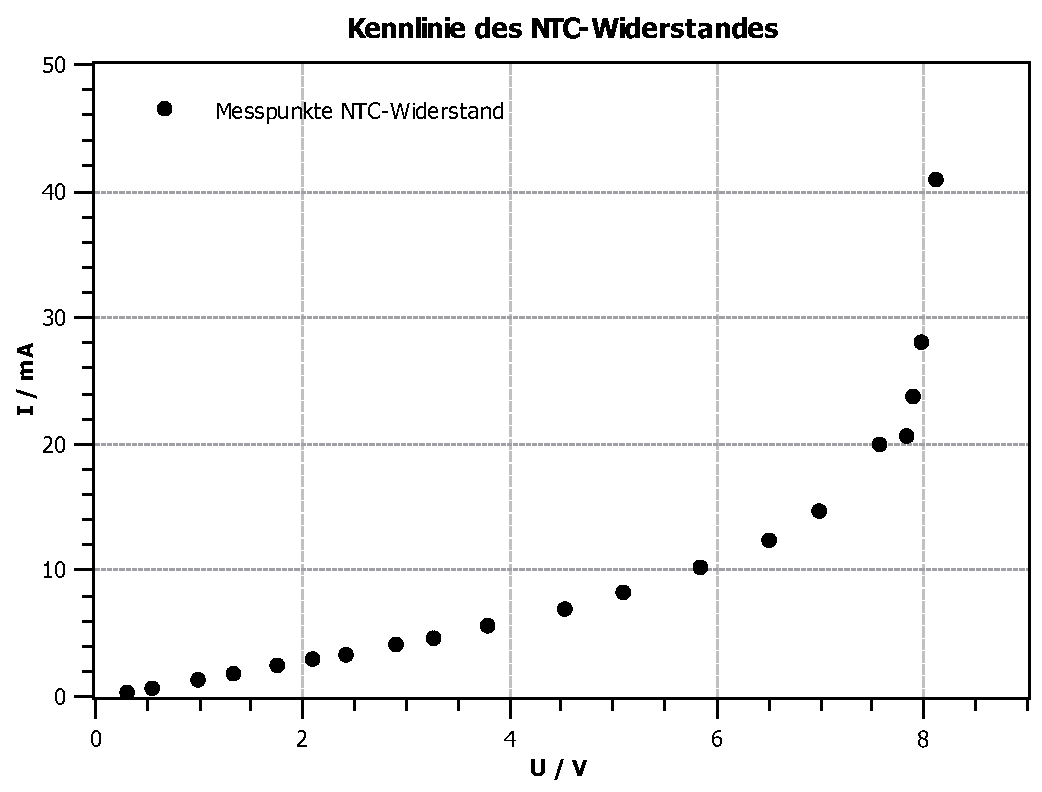
\includegraphics[width=\textwidth]{KennlinieNTCsubgitter.pdf}
					\caption{Messung zu Versuch 1d)}
					\label{KL d}
				\end{figure}
			
			\subsubsection*{Schlussfolgerung}
			
				Hier ist klar zu erkennen, dass der Widerstand mit steigender Temperatur (durch steigende Ströme) sinkt, was für NTC-Widerstände charakteristisch ist. 
				Dass wir auch hier nicht höhere Eingangsspannungen als \SI{8}{\V} einstellen konnten, könnte auch hier an dem Innenwiderstand des Netzteils gelegen haben.
			
		\subsection{e) Glimmlampe} 
			
			Bei der Glimmlampe kann der Strom nicht einfach durchfließen, da kein elektrischer Leiter die beiden Pole direkt miteinander verbindet.
			Damit ein Strom fließen kann, muss er von der Kathode zur Anode gelangen.
			Zwischen den beiden befindet sich lediglich ein Gas, welches als Leiter dienen soll.
			Dieses kann jedoch nur durch Gasentladungen den elektrischen Strom von der Kathode zur Anode führen.
			
			\subsubsection*{Gasentladungen}
			
				Die an der Kathode anliegende Spannung setzt Elektronen aus dieser frei.

				Je höher die anliegende Spannung, desto schneller werden die Elektronen beschleunigt und erreichen bei der Anode eine höhere Maximalgeschwindigkeit und somit eine größere Energie.
				Sind sie schnell genug um die Gasatome durch Stoßionisation anzuregen, führt dies zu einer Kettenreaktion von sich lösenden Elektronen.
				Die Spannung, welche man für Anregung der Gasatome braucht, nennt man Zündspannung. 
				
				An der Anode kommen schließlich, aus den Gasatomen gelöste, Elektronen an und ein Strom fließt, solange die Ionisation des Gases aufrecht erhalten wird.
				Sinkt die Spannung unter die sogenannte Löschspannung, dann ist dies nicht mehr möglich und die Entladung wird unterbrochen.

				Die Löschspannung ist geringer als die Zündspannung, da die Energie nach erstmaliger Ionisation nur noch für die Anregung benötigt wird.
					
				Zudem wird Licht bei der Ionisation des Gases bzw. dem Zurückfallen der Elektronen emittiert, was das \glqq Glimmen\grqq{} der Lampe ausmacht.
				
			\subsubsection*{Messung}
			
				Wir messen zunächst, welche Spannung notwendig ist, um die Glimmlampe zu zünden.
				Für diese Zündspannung haben wir einen Wert von ca. \SI{119}{\V} gemessen.
				Danach fiel die von uns gemessene Eingangsspannung instantan auf ca. \SI{88,4}{\V} ab und wir haben einen Strom gemessen.
				Hier fing die Glimmlampe auch an zu leuchten.
				Bis zum Erreichen der Zündspannung war dieser Strom gleich null, weswegen wir nur den relevanten Bereich in Abb. \ref{KL e} dargestellt haben.
				
				Wir haben zunächst versucht die Eingangsspannung zu erhöhen, was bis zu ca. \SI{92}{\V} möglich war. In diesem Bereich sieht das Strom-Spannungs-Verhältnis nahezu linear aus.
				
				Das Herunterregeln der Eingangsspannung ergab unerwartete Effekte. Wie zum Beispiel, dass das dieses teilweise zu höheren Spannungen an der Glimmlampe geführt hat.				
				Der Strom hingegen wurde mit dem Herunterregeln kleiner bis wir schließlich eine Stromstärke von null erreicht haben\footnote{siehe dazu Reihenfolge der Messwerte im Laborbuch, Seite 2}.

				Nachdem die Glimmlampe erlischt war, musste die Zündspannung ein weiteres Mal angelegt werden, um sie zu entzünden.
			
				\begin{figure}
					\centering
					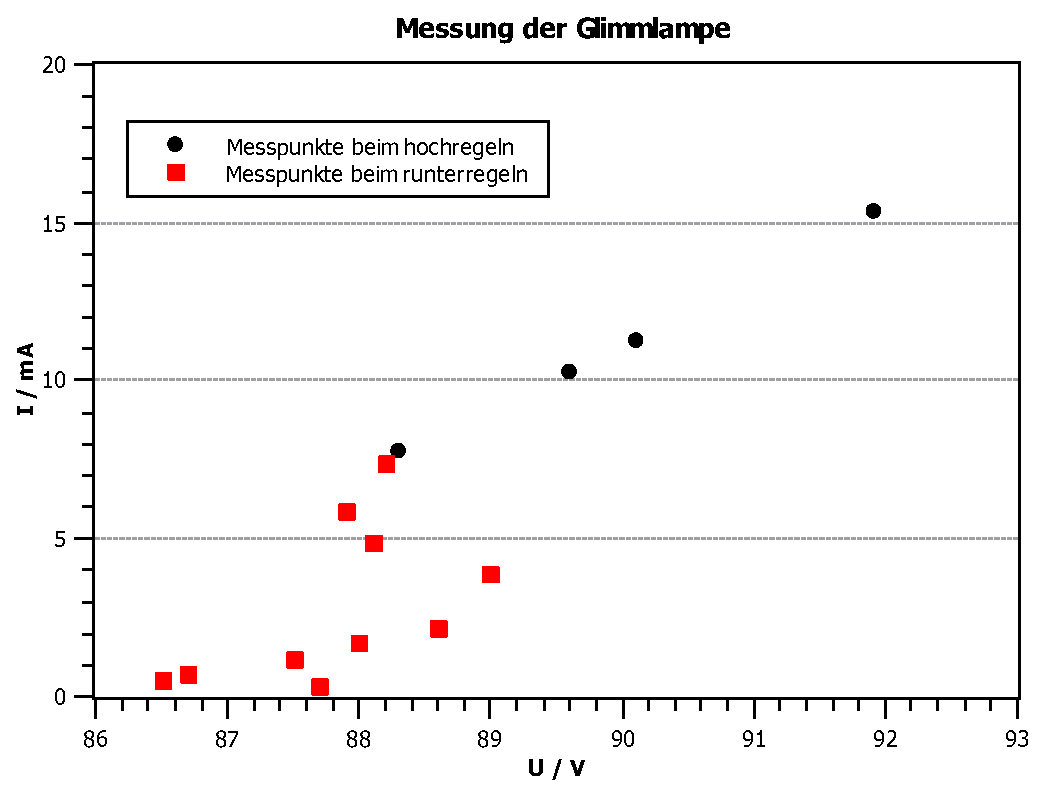
\includegraphics[width=\textwidth]{KennlinieGlimmlampe.pdf}
					\caption{Messung zu Versuch 1e)}
					\label{KL e}
				\end{figure}
			
			\subsubsection*{Schlussfolgerung}
			
				Wir entnehmen unserer Messung, dass die Zündspannung der Glimmlampe bei ca. \SI{119}{\V} liegt.
				
				Die Löschspannung liegt zwischen \SI{86,5}{\V} und \SI{88}{\V}. Sie konnte nicht eindeutig festgelegt werden, da zwar bei \SI{87,7}{\V} die Lampe erlischt, es jedoch auch niedrigere Spannungen gab, bei denen die Lampe noch geleuchtet hat.
				
				Für die Zündspannung wurde uns ein Wert von ungefähr \SI{120}{\V} vorgegeben, welcher mit unserer Messung weitgehend übereinstimmt, lediglich eine Differenz von \SI{1}{\V}.
					
	\newpage	
	\section{Versuch 2: Widerstand in Abhängigkeit der Temperatur}		
		
		In diesem Versuch beschäftigen wir uns mit der Leitfähigkeit eines Kupferdrahtes in Abhängigkeit der Temperatur.
		
		\subsection{Methoden} 
		
			Wir schließen unseren Kupferdraht an eine Wheatstone'sche Brückenschaltung an (siehe Abb. \ref{Schaltskizze2}). Hierbei bezeichnet $R_\text{x}(T)$ unseren Kupferdraht, $R_\text{v}$ einen einfachen \SI{5}{\Omega} Widerstand und $R_\text{e}$ den \SI{11,3}{\Omega} Widerstand, welcher sich wie ein Potentiometer einstellen lässt. Bei diesem handelt es sich um einen Widerstand über ein Metall. Widerstände dieser Art sind proportional zur Länge $l$ des Metalls und antiproportional zur ihrer Querschnittsfläche $A$. 
			
			\begin{equation*}
				R = \varrho \frac{l}{A} \Rightarrow R_e(x) = \frac{x}{l} R_0 = \SI{11,3} x \cdot \si{\Omega\per\meter}
			\end{equation*}				
			$x$ sei hierbei die Position des Schiebereglers und $l$ die gesammte Länge des Drahtes.	
			
			Das Prinzip der Wheatstone'schen Brücke ermöglicht uns mit Hilfe der Kirchhoff'schen Regeln einen unbekannten Widerstand zu berechnen.
			Wird an dem Strommessgerät, wie es in Abb. \ref{Schaltskizze2} verbaut ist, kein Strom gemessen, dann gilt nach dem Abgleichverfahren
			\begin{equation*}
				\frac{R_e(x)}{R_0-R_e(x)} = \frac{R_\nu}{R_x} \Rightarrow R_x = \frac{x}{l-x} R_\nu.
			\end{equation*}
			Wir stellen unseren Widerstand $R_\text{e}$ über den Schieberegler also für jede Messung so ein, dass $I = 0$ erfüllt ist. Es wird erst über den \SI{20}{k\Omega} kalibriert und dann über den geschlossenem Schalter für genauere Messungen.
			
			Bevor wir die Messung beginnen, kühlen wir unseren Draht auf ca. \SI{0}{\celsius} ab.
			Nun erhitzen wir ihn langsam auf nahezu \SI{100}{\celsius} und messen währenddessen kontinuierlich die Temperatur und die Position des Schiebereglers.
			Das gleiche wiederholen wir für die Abkühlung bis \SI{15}{\celsius}, wobei wir Eis genutzt haben, um den Prozess etwas zu beschleunigen.
						
			\begin{figure}
				\centering
				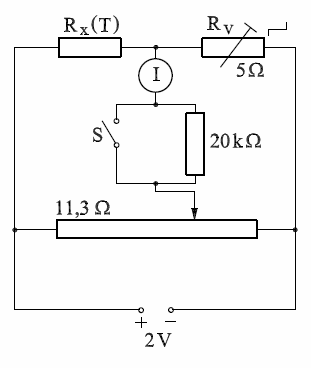
\includegraphics[width=0.6\textwidth]{Versuch2.png}
				\caption{Schaltskizze zu Versuch 1}
				\label{Schaltskizze2}
			\end{figure}
		
		\subsection{Messung}
			
			Abb. \ref{Ölbad} stellt die Position des Widerstandreglers in Abhängigkeit von der Temperatur dar.
			Die Gesamtlänge des Widerstands liegt bei \SI{100}{cm}.
			
			In Abb. \ref{fig:drahtRT} sind die umgerechneten Widerstände gegen die Temperatur aufgetragen.
			Die Ausgleichsgerade hat eine Steigung von $m = 0,021335$ und schneidet die y-Achse bei $y_0 = 5,005$.
			
			\begin{figure}
				\centering
				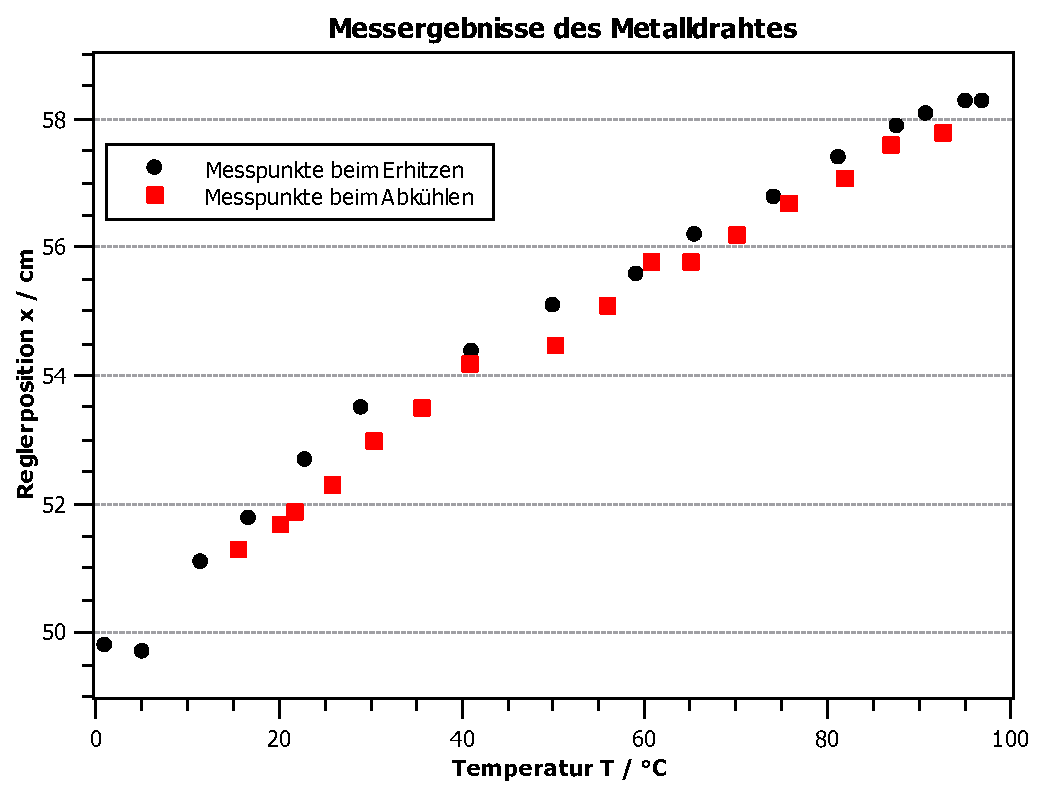
\includegraphics[width=\textwidth]{MessungDraht.pdf}
				\caption{Position des Widerstandreglers in Abhängigkeit von der Temperatur}
				\label{Ölbad}
			\end{figure}
			\begin{figure}
				\centering
				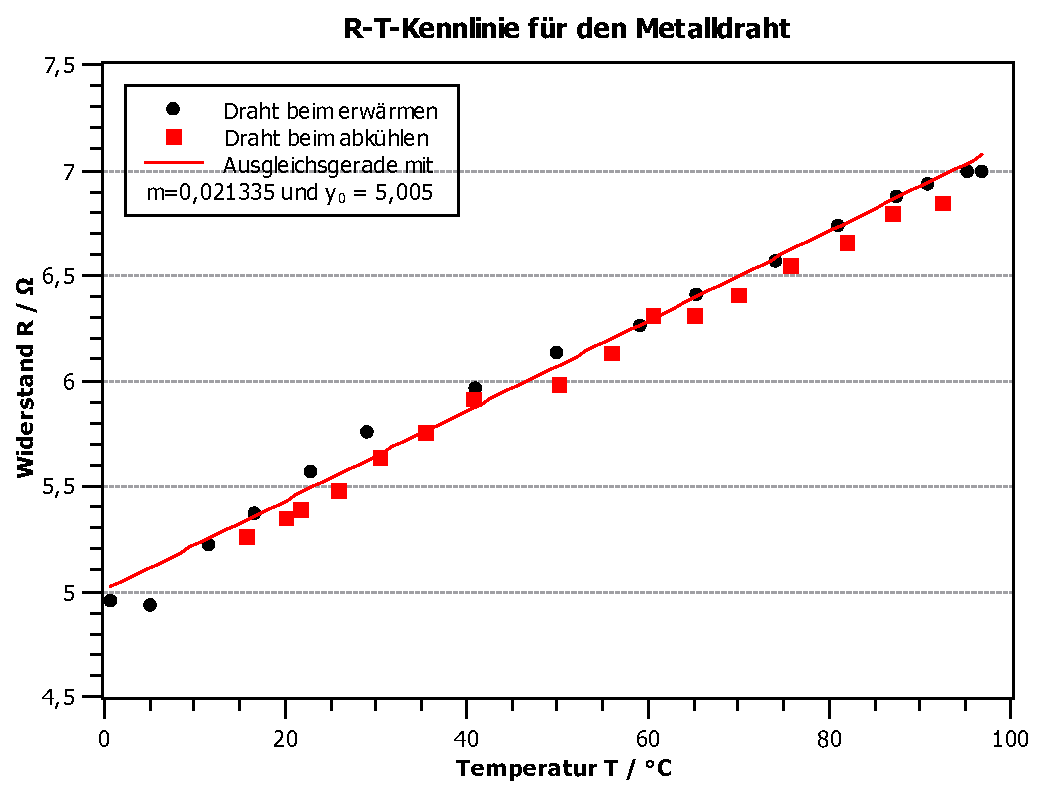
\includegraphics[width=\textwidth]{KennlinieDrahtRT.pdf}
				\caption{Widerstand des Drahtes relativ zur Temperatur}
				\label{fig:drahtRT}
			\end{figure}
			
		\subsection{Schlussfolgerung}	
			
			Wie auch schon bei der Glühlampe erkennen wir, dass die Eigenschaft eines Metallleiters, mit steigender Temperatur schlechter den elektrischen Strom zu leiten, von dem Kupferdraht erfüllt wird.
			
			Entgegen der Erwartung ist der Widerstand des Drahtes nicht vorgelaufen, sondern eher im Gegenteil zurückgeblieben.
			Das sieht man z. B. in {Abb. \ref{fig:drahtRT}} gut daran, dass die meisten Werte beim erwärmen über der Geraden liegen, während sie beim abkühlen größtenteils unter dieser sind.
			
			Der Temperaturkoeffizient $\alpha$ ist gerade die Steigung $m$ der Ausgleichsgerade.
			Also $\alpha = 0,021335$.
		
	\begin{thebibliography}	
		e Abbildungen \ref{Schaltskizze1} und \ref{Schaltskizze2} wurden der Versuchsanleitung entnommen
	\end{thebibliography}	
			
\end{document} 